\documentclass[tikz, crop, border = {2pt 2pt 2pt 2pt}]{standalone}

\usepackage{physics}
\usepackage{concmath-otf}
\usetikzlibrary{decorations.pathreplacing}

\begin{document}

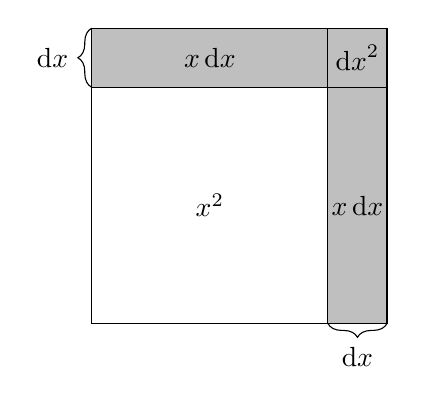
\begin{tikzpicture}
    \draw (0, 0) rectangle (3, 3) node[midway]{$x^2$};
    \draw (0, 0) rectangle (3.75, 3.75);
    \draw (3, 3) -- (3.75, 3) (3.75, 3.75) -- (3, 3.75);
    \filldraw[draw = black, fill = lightgray] (3, 3) rectangle (3.75, 3.75) node[midway]{$\dd{x}^2$};
    \filldraw[draw = black, fill = lightgray] (3, 0) rectangle ++ (0.75, 3) node[midway]{$x\dd{x}$};
    \filldraw[draw = black, fill = lightgray] (0, 3) rectangle ++ (3, 0.75) node[midway]{$x\dd{x}$};

    \draw[decorate, decoration = {brace, amplitude = 5pt, mirror}] (3, 0) -- ++ (0.75, 0) node[midway, below = 5pt]{$\dd{x}$};
    \draw[decorate, decoration = {brace, amplitude = 5pt}] (0, 3) -- ++ (0, 0.75) node[midway, left = 5pt]{$\dd{x}$};
\end{tikzpicture}

\end{document}